\documentclass[spanish,a4paper,11pt,twoside]{report}

%%%%%%%%%%%%%%%%%%%%%%%%%%%%%%%%%%%%%%%%%%%%%%%%%%%%%%%%%%%%%%%%%%%%%%%%%%%%%%%
\usepackage[dvips]{graphicx}
\usepackage[dvips]{epsfig}
\usepackage[latin1]{inputenc}
\usepackage[spanish]{babel}
\usepackage{alltt}
\usepackage{templates/algorithm}
\usepackage{templates/algorithmic}
\usepackage{templates/multirow}

%%%%%%%%%%%%%%%%%%%%%%%%%%%%%%%%%%%%%%%%%%%%%%%%%%%%%%%%%%%%%%%%%%%%%%%%%%%%%%%

\newcommand{\SONY}{{\sc Sony}}
\newcommand{\MICROSOFT}{{\sc Microsoft}}
\newcommand{\GCC}{\textsf{\textsc{G}CC}}
\newcommand{\INTEL}{\textsf{\textsc{I}ntel}}

%%% Traducimos el pseudocodigo
\renewcommand{\algorithmicwhile}{\textbf{mientras}}
\renewcommand{\algorithmicend}{\textbf{fin}}
\renewcommand{\algorithmicdo}{\textbf{hacer}}
\renewcommand{\algorithmicif}{\textbf{si}}
\renewcommand{\algorithmicthen}{\textbf{entonces}}
\renewcommand{\algorithmicrepeat}{\textbf{repetir}}
\renewcommand{\algorithmicuntil}{\textbf{hasta que}}
\renewcommand{\algorithmicelse}{\textbf{en otro caso}}
\renewcommand{\algorithmicfor}{\textbf{para}}

%\newcommand{\RETURN}{\textbf{retornar} }
\newcommand{\RET}{\STATE \textbf{retornar} }
\newcommand{\TO}{\textbf{hasta} }
\newcommand{\AND}{\textbf{y} }
\newcommand{\OR}{\textbf{o} }

%%%%%%%%%%%%%%%%% Creamos un entorno para listar c�digo fuente %%%%%%%%%%%%%%%
\newenvironment{sourcecode}
{\begin{list}{}{\setlength{\leftmargin}{1em}}\item\scriptsize\bfseries}
{\end{list}}

\newenvironment{littlesourcecode}
{\begin{list}{}{\setlength{\leftmargin}{1em}}\item\tiny\bfseries}
{\end{list}}

\newenvironment{summary}
{\par\noindent\begin{center}\textbf{Abstract}\end{center}\begin{itshape}\par\noindent}
{\end{itshape}}

\newenvironment{keywords}
{\begin{list}{}{\setlength{\leftmargin}{1em}}\item[\hskip\labelsep \bfseries Keywords:]}
{\end{list}}

\newenvironment{palabrasClave}
{\begin{list}{}{\setlength{\leftmargin}{1em}}\item[\hskip\labelsep \bfseries Palabras clave:]}
{\end{list}}


%%%%%%%%%%%%%%%%%%%%%%%%%%%%%%%%%%%%%%%%%%%%%%%%%%%%%%%%%%%%%%%%%%%%%%%%%%%%%%%
% Format
%%%%%%%%%%%%%%%%%%%%%%%%%%%%%%%%%%%%%%%%%%%%%%%%%%%%%%%%%%%%%%%%%%%%%%%%%%%%%%%

%%\topmargin -4 mm
%\topmargin -21 mm
%\headheight 10 mm
%\headsep 10 mm

%\textheight 229 mm
%\textheight 246 mm

%\oddsidemargin -5.4 mm
%\evensidemargin -5.4 mm
\oddsidemargin 5 mm
\evensidemargin 5 mm

%\oddsidemargin -3 mm
%\evensidemargin -3 mm

%\textwidth 17 cm
\textwidth 15 cm
%\columnsep 10 mm

\input{amssym.def}

%%%%%%%%%%%%%%%%%%%%%%%%%%%%%%%%%%%%%%%%%%%%%%%%%%%%%%%%%%%%%%%%%%%%%%%%%%%%%%%

\begin{document}

%%%%%%%%%%%%%%%%%%%%%%%%%%%%%%%%%%%%%%%%%%%%%%%%%%%%%%%%%%%%%%%%%%%%%%%%%%%%%%%
% First Page 
%%%%%%%%%%%%%%%%%%%%%%%%%%%%%%%%%%%%%%%%%%%%%%%%%%%%%%%%%%%%%%%%%%%%%%%%%%%%%%%

\pagestyle{empty}
\thispagestyle{empty}


\newcommand{\HRule}{\rule{\linewidth}{1mm}}
\setlength{\parindent}{0mm}
\setlength{\parskip}{0mm}
\vspace*{\stretch{1}}

\begin{center}

\includegraphics[width=0.2\textwidth]{images/logotipo-secundario-ULL}\\[0.25cm]
\end{center}

\HRule
\begin{center}
        {\Huge T�tulo del trabajo} \\[2.5mm] 
        {\Huge Subt�tulo} \\[2.5mm]
        {\Large Autor (o autores)} \\[5mm]
        {\Large \textit{Grupo ($1\mid2$) }} \\[5mm]


        {\em T�cnicas Experimentales. $1^{er}$ curso. $2^{do}$ semestre} \\[5mm]
        Lenguajes y Sistemas Inform�ticos \\[5mm]
        Facultad de Matem�ticas \\[5mm]
        
        Universidad de La Laguna \\
\end{center}
\HRule
\vspace*{\stretch{2}}
\begin{center}
  La Laguna, \today 
\end{center}

%%%%%%%%%%%%%%%%%%%%%%%%%%%%%%%%%%%%%%%%%%%%%%%%%%%%%%%%%%%%%%%%%%%%%%%%%%%%%%%

%%%%%%%%%%%%%%%%%%%%%%%%%%%%%%%%%%%%%%%%%%%%%%%%%%%%%%%%%%%%%%%%%%%%%%%%%%%%%%%
\newpage{\pagestyle{empty}\cleardoublepage}

\pagestyle{myheadings} %my head defined by markboth or markright
% No funciona bien \markboth sin "twoside" en \documentclass, pero al
% ponerlo se dan un mont�n de errores de underfull \vbox, con lo que no se
% ha puesto.
\markboth{Nombre del alumno}{T�tulo del trabajo}

%%%%%%%%%%%%%%%%%%%%%%%%%%%%%%%%%%%%%%%%%%%%%%%%%%%%%%%%%%%%%%%%%%%%%%%%%%%%%%%
%Numeracion en romanos
\renewcommand{\thepage}{\roman{page}}
\setcounter{page}{1}

%%%%%%%%%%%%%%%%%%%%%%%%%%%%%%%%%%%%%%%%%%%%%%%%%%%%%%%%%%%%%%%%%%%%%%%%%%%%%%%

\tableofcontents

%%%%%%%%%%%%%%%%%%%%%%%%%%%%%%%%%%%%%%%%%%%%%%%%%%%%%%%%%%%%%%%%%%%%%%%%%%%%%%%
\newpage{\pagestyle{empty}\cleardoublepage}

\listoffigures

%%%%%%%%%%%%%%%%%%%%%%%%%%%%%%%%%%%%%%%%%%%%%%%%%%%%%%%%%%%%%%%%%%%%%%%%%%%%%%%
\newpage{\pagestyle{empty}\cleardoublepage}

\listoftables

%%%%%%%%%%%%%%%%%%%%%%%%%%%%%%%%%%%%%%%%%%%%%%%%%%%%%%%%%%%%%%%%%%%%%%%%%%%%%%%
\newpage{\pagestyle{empty}\cleardoublepage}

%%%%%%%%%%%%%%%%%%%%%%%%%%%%%%%%%%%%%%%%%%%%%%%%%%%%%%%%%%%%%%%%%%%%%%%%%%%%%%%
%Numeracion a partir del capitulo I
\renewcommand{\thepage}{\arabic{page}}
\setcounter{page}{1}

\setlength{\parindent}{5mm}

%%%%%%%%%%%%%%%%%%%%%%%%%%%%%%%%%%%%%%%%%%%%%%%%%%%%%%%%%%%%%%%%%%%%%%%%%%%%%%%
\chapter{Motivaci�n y objetivos}
\label{chapter:obj}

%%%%%%%%%%%%%%%%%%%%%%%%%%%%%%%%%%%%%%%%%%%%%%%%%%%%%%%%%%%%%%%%%%%%%%%%%%%%%
% Chapter 1: Motivaci�n y Objetivos 
%%%%%%%%%%%%%%%%%%%%%%%%%%%%%%%%%%%%%%%%%%%%%%%%%%%%%%%%%%%%%%%%%%%%%%%%%%%%%%%


%---------------------------------------------------------------------------------
\section{Motivaci�n}
\label{1:sec:1}
\begin{itemize}
  \item	 Familiarizaci�n con la creaci�n de informes cient�ficos.
	Esta tarea nos aportar� unas nociones b�sicas que nos ayudar�n en el transcurso de nuestra carrera. Ser� importante su correcto aprendizaje para el futoro, esto se debe a que jugar� un papel importante en el trabajo de fin de grado.
  \item  Correcto aprendizaje de diversas herramientas:
	\begin{itemize}
	 \item	\LaTeX{}
	 \item	Beamer
	 \item	Python
	\end{itemize}
\end{itemize}


%---------------------------------------------------------------------------------
\section{Objetivos}
\label{1:sec:2}
  El trabajo se ha realizado con los objetivos siguientes:

\begin{itemize}
  \item  Aprender a buscar informaci�n adecuada para el desarrollo de la tarea a realizar. Utilizando, entre otras cosas, las herramientas de la BULL.
  \item  Analizar el problema a estudiar y dise�ar una soluci�n a dicho problema.
  \item  Crear e implementar un algoritmo de resoluci�n al problema dado mediante Python.
  \item  Verificar mediante pruebas que la soluci�n propuesta es correcta y eficiente.
  \item  Elaborar un informe final sobre el tema utilizando \LaTeX{}
  \item  Realizar una presentaci�n p�blica del mismo.
\end{itemize}



%%%%%%%%%%%%%%%%%%%%%%%%%%%%%%%%%%%%%%%%%%%%%%%%%%%%%%%%%%%%%%%%%%%%%%%%%%%%%%%
\chapter{Fundamentos te�ricos}
\label{chapter:teo}

%%%%%%%%%%%%%%%%%%%%%%%%%%%%%%%%%%%%%%%%%%%%%%%%%%%%%%%%%%%%%%%%%%%%%%%%%%%%%%%
% Chapter 2: Fundamentos Te�ricos 
%%%%%%%%%%%%%%%%%%%%%%%%%%%%%%%%%%%%%%%%%%%%%%%%%%%%%%%%%%%%%%%%%%%%%%%%%%%%%%%

%++++++++++++++++++++++++++++++++++++++++++++++++++++++++++++++++++++++++++++++
%++++++++++++++++++++++++++++++++++++++++++++++++++++++++++++++++++++++++++++++

\section{¿Quien fue Taylor?}
\label{2:sec:1}
  Brook Taylor fue un matem\'atico brit\'anico naci\'o en Edmonton, Middlesex el 18 de agosto de 1685, en el seno de una familia noble.\\
Taylor cont\'o con una esmerada educaci\'on impartida por tutores privados hasta que se matricul\'o en el St. John's College de Cambridge. Con 24 a\~nos se licenci\'o en Derecho, y a los 29 se doctor\'o en esta materia. Pero es dudoso que alguna vez llegara a ejercer como abogado, ya que lo que verdaderamente le gustaba eran las matem\'aticas, que estudi\'o con John Machin y John Keill.\\
Su primer trabajo matem\'atico importante fue en 1708 la soluci\'on al problema del "centro de oscilaci\'on" que, sin embargo, no se publicar\'ia hasta seis a\~nos en la revista Transacciones Filos\'oficas de la Royal Society, lo que provoc\'o una disputa sobre su autor\'ia con Johann Bernoulli.\\
En 1712 fue elegido miembro de esa prestigiosa sociedad, y form\'o parte de la comisi\'on que deb\'ia juzgar si la autor\'ia del calculo diferencial correspond\'ia a Newton o a Leibniz. Fueron habituales los art\'iculos en la revista de la Sociedad, en los que, entre otras cosas, analiz\'o el movimiento de los proyectiles, las formas adoptadas por los l\'iquidos, los fen\'omenos de capilaridad, interesantes experimentos sobre el magnetismo o una nueva forma de c\'alculo para aproximar las ra\'ices de una ecuaci\'on dando lugar a un m\'etodo nuevo para logaritmos computacionales.\\
En 1721 se cas\'o con una chica de buena familia pero sin dinero, lo que le llev\'o a enemistarse con su padre, que no ve\'ia con buenos ojos el matrimonio. La enemistad acab\'o en 1723 con la muerte de su mujer durante el parto, en el que tambi\'en muri\'o el ni\~no. Dos a\~nos m\'as tarde contraer\'ia de nuevo matrimonio, esta vez con la bendici\'on paterna, con Sabetta Sawbridge, que tambi\'en muri\'o de parto en 1730. Pero en este caso, su hija sobrevivi\'o.
Taylor nunca, hab\'ia gozado de buena salud, y despu\'es de enviudar por segunda vez su estado se deterior\'o r\'apidamente. Muri\'o en Somerset House, cerca de Londres, el 29 de diciembre de 1731, a los 46 a\~nos de edad.

\section{Aportaciones de Taylor a las Matem\'aticas}
\label{2:sec:2}
  En su obra m\'as famosa, Methodus Incrementorum Directa et Inversa, en 1715, desarroll\'o una nueva rama de las matem\'aticas conocida como C\'alculo de las diferencias finitas. En ella estudi\'o los cambios de variable, las diferencias finitas (las cuales defini\'o como incrementos), y present\'o el desarrollo en una serie de una funci\'on de una variable.
Con este m\'etodo pudo determinar la ecuaci\'on diferencial que explica el movimiento de una cuerda vibrante, y trazar la trayectoria curva que sigue un rayo de luz cuando atraviesa un medio heterog\'eneo como la atm\'osfera.\\
La obra tambi\'en contiene la famosa f\'ormula conocida como el Teorema de Taylor, cuya gran importancia para el desarrollo del c\'alculo diferencial fue puesta de manifiesto sesenta a\~nos despu\'es por el matem\'atico franc\'es Lagrange.
Se trata de uno de los mayores inventos de la humanidad, pues permite reducir c\'alculos con funciones complicadas a las operaciones aritm\'eticas elementales suma y multiplicaci\'on.\\
En otra de sus obras, Ensayo sobre la perspectiva lineal, Taylor estableci\'o las bases de la perspectiva geom\'etrica e introdujo el principio de los puntos dispersos.
También destaca su correspondencia con Pierre R\'emond de Montmort sobre las doctrinas de Nicolas Malebranche. Entre sus cartas y tratados inacabados se han encontrado escritos sobre los sacrificios hebreos y sobre la legitimidad de comer sangre.\\
Fue un cient\'ifico formidable, capaz de competir con matem\'aticos de la talla de Johann Bernoulli.
Sin embargo, gran parte de sus descubrimientos no tuvieron repercusi\'on o se perdieron a causa de su incapacidad de expresar sus ideas completamente y con claridad.\\

Un trabajo p\'ostumo titulado Contemplaci\'on Filos\'ofica, fue publicado en 1793 por su sobrino, William Young.
\subsection{Interpolaci\'on por Taylor}
Dada una funci\'on $f$ de la cual se conocen sus valores en un n\'umero finito de abscisas $x_{0}, x_{1}, ..., x_{m}$, se llama interpolaci\'on polin\'omica al proceso de hallar un polinomio $p_{m}(x)$ de grado menor o igual a $m$, cumpliendo $p_{m}(x_{k}) = f(x_{k})$, $\forall k = 0, 1, ..., m$
A este polinomio se le llama Polinomio interpolador de grado m de la funci\'on $f$.\\
\\
El problema de Interpolaci\'on de Taylor tiene soluci\'on \'unica, que se denomina polinomio de Taylor de grado menos o igual a n de la funci\'on f en el punto $x_{0}$:
$$p(x)=f(x_{0})+f'(x_{0})(x-x_{0})+f''(x_{0})\frac{(x-x_{0})^2}{2!}+...+f^{(n)}(x_{0})\frac{(x-x_{0})^n}{n!}$$


%%%%%%%%%%%%%%%%%%%%%%%%%%%%%%%%%%%%%%%%%%%%%%%%%%%%%%%%%%%%%%%%%%%%%%%%%%%%%%%
\chapter{Procedimiento experimental}
\label{chapter:exp}


\section{Descripci\'on de los experimentos}
\label{3:sec:1}


\section{Descripci\'on del material}
\label{3:sec:2}
Para la realizaci\'on de las pruebas efectuadas se ha utilizado una m\'aquina computacional (ordenador) con las siguientes caracter\'isticas:\\
\begin{itemize}
 \item CPU type: Intel(R) Core(TM) i5 CPU M 460  @ 2.53GHz 
 \item Vendor ID: GenuineIntel
 \item CPU speed: 1199.000 Hz
 \item Cache size: 3072 KB
\end{itemize}



%++++++++++++++++++++++++++++++++++++++++++++++++++++++++++++++++++++++++++++++
\section{Resultados obtenidos}
\label{3:sec:3}

bla, bla, etc. 


%------------------------------------------------------------------------------
\begin{figure}[!th]
\begin{center}
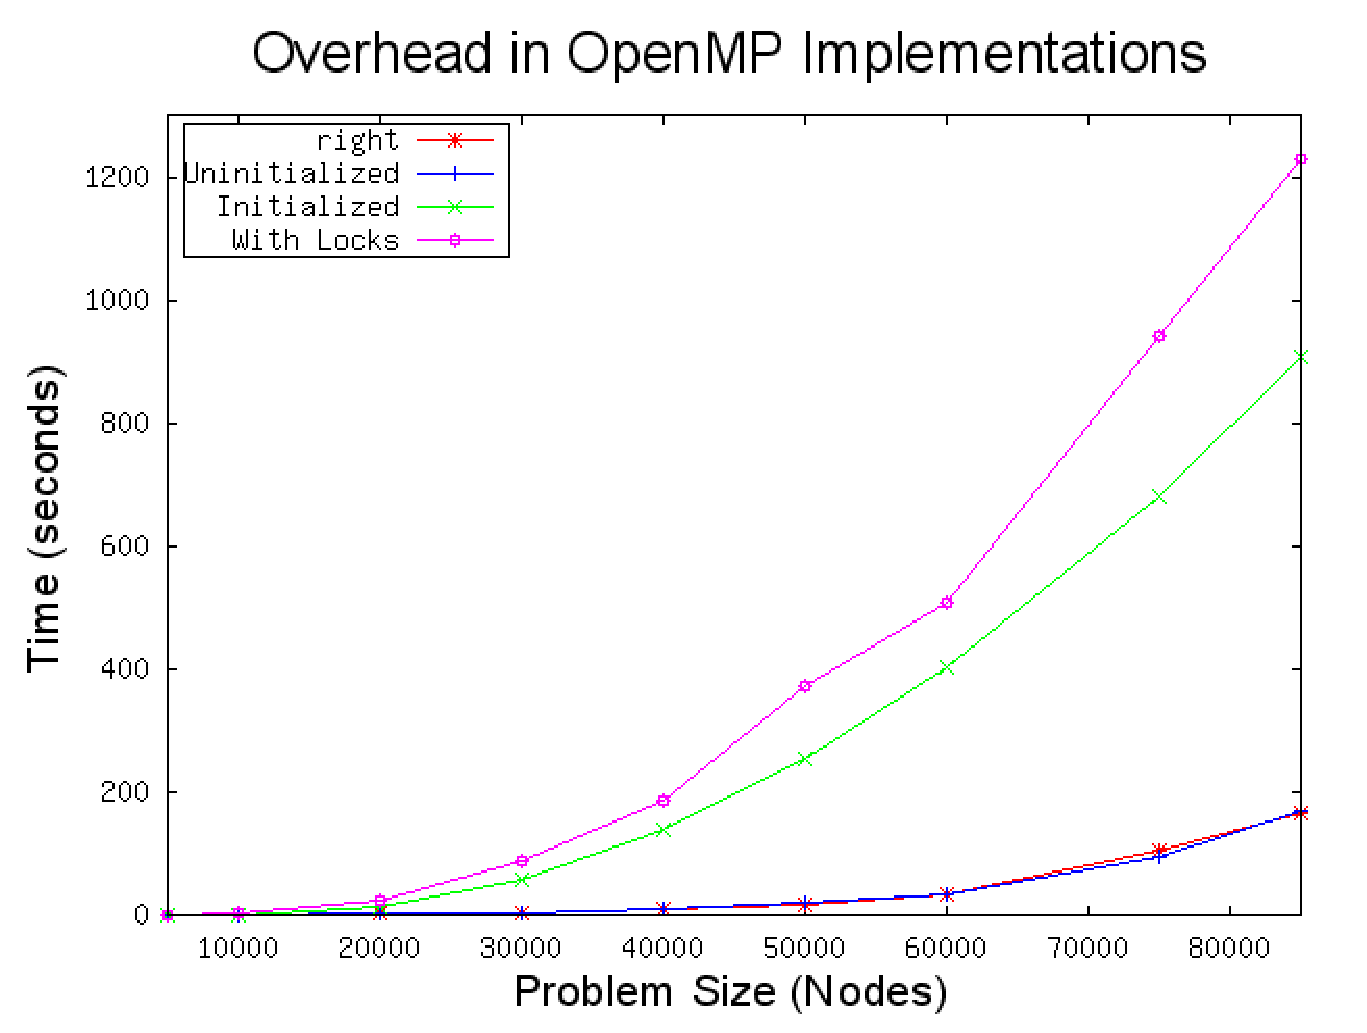
\includegraphics[width=0.75\textwidth]{images/figura1.eps}
\caption{Ejemplo de figura}
\label{fig:1}
\end{center}
\end{figure}
%------------------------------------------------------------------------------


%------------------------------------------------------------------------------
%--------------------------------------------------------------------------
\begin{table}[!ht]
\begin{center}
\begin{tabular}{|c|c|} \hline 
\textbf{Tiempo  } & \textbf{Velocidad} \\ 
\textbf{($\pm$ 0.001 s)} & \textbf{($\pm$ 0.1 m/s)} \\ \hline \hline
1.234 &
67.8
\\
\hline

2.345 &
78.9
\\
\hline

3.456 &
89.1
\\
\hline

4.567 &
91.2
\\
\hline

\end{tabular}
\end{center}
\caption{Resultados experimentales de tiempo (s) y velocidad (m/s)}
\label{tab:1}
\end{table}


%------------------------------------------------------------------------------

%++++++++++++++++++++++++++++++++++++++++++++++++++++++++++++++++++++++++++++++
\section{An�lisis de los resultados}
\label{3:sec:4}

bla, bla, etc. 

%%%%%%%%%%%%%%%%%%%%%%%%%%%%%%%%%%%%%%%%%%%%%%%%%%%%%%%%%%%%%%%%%%%%%%%%%%%%%%%
\chapter{Conclusiones}
\label{chapter:conclusiones}

%%%%%%%%%%%%%%%%%%%%%%%%%%%%%%%%%%%%%%%%%%%%%%%%%%%%%%%%%%%%%%%%%%%%%%%%%%%%%
% Chapter 4: Conclusiones y Trabajos Futuros 
%%%%%%%%%%%%%%%%%%%%%%%%%%%%%%%%%%%%%%%%%%%%%%%%%%%%%%%%%%%%%%%%%%%%%%%%%%%%%%%

bla, bla, bla, etc.


%%%%%%%%%%%%%%%%%%%%%%%%%%%%%%%%%%%%%%%%%%%%%%%%%%%%%%%%%%%%%%%%%%%%%%%%%%%%%%%

%%%%%%%%%%%%%%%%%%%%%%%%%%%%%%%%%%%%%%%%%%%%%%%%%%%%%%%%%%%%%%%%%%%%%%%%%%%%%%%
\newpage{\pagestyle{empty}\cleardoublepage}
\thispagestyle{empty}
\begin{appendix}

\chapter{T�tulo del Ap�ndice 1}
\label{appendix:1}

\section{Algoritmo XXX}
\label{Apendice1:XXX}

\begin{center}
\begin{footnotesize}
\begin{verbatim}
###################################################################################
# Fichero .py
###################################################################################
#
# AUTORES
#   
# FECHA
#
# DESCRIPCION
#
###################################################################################
\end{verbatim}
\end{footnotesize}
\end{center}

\section{Algoritmo YYY}
\label{Apendice1:YYY}

\begin{center}
\begin{footnotesize}
\begin{verbatim}
/###################################################################################
 # Fichero .h
 ###################################################################################
 #
 # AUTORES
 #
 # FECHA
 #
 # DESCRIPCION
 #
 ##################################################################################
\end{verbatim}
\end{footnotesize}
\end{center}


\chapter{T�tulo del Ap�ndice 2}
\label{appendix:2}

\section{Otro apendice: Seccion 1}
\label{Apendice2:label}

\begin{center}
\begin{footnotesize}

\begin{verbatim}
Texto
\end{verbatim}

\end{footnotesize}
\end{center}

\section{Otro apendice: Seccion 2}
\label{Apendice2:label2}

\begin{center}
\begin{footnotesize}

\begin{verbatim}
Texto
\end{verbatim}


\end{footnotesize}
\end{center}


\end{appendix}

%%%%%%%%%%%%%%%%%%%%%%%%%%%%%%%%%%%%%%%%%%%%%%%%%%%%%%%%%%%%%%%%%%%%%%%%%%%%%%%
\addcontentsline{toc}{chapter}{Bibliograf�a}
\bibliographystyle{plain}


\bibliography{bib/references}
\nocite{*}

%%%%%%%%%%%%%%%%%%%%%%%%%%%%%%%%%%%%%%%%%%%%%%%%%%%%%%%%%%%%%%%%%%%%%%%%%%%%%%%

\end{document}
